
%%%%%%%%%%%%%%%%%%%%%%%%%%%%%%%%%%%%%%%%%%%%%%%%%%%%%%%%
%
% Copyright (c) 2003-2009 by University of Queensland
% Earth Systems Science Computational Center (ESSCC)
% http://www.uq.edu.au/esscc
%
% Primary Business: Queensland, Australia
% Licensed under the Open Software License version 3.0
% http://www.opensource.org/licenses/osl-3.0.php
%
%%%%%%%%%%%%%%%%%%%%%%%%%%%%%%%%%%%%%%%%%%%%%%%%%%%%%%%%


\section{Elastic Deformation}
\label{ELASTIC CHAP}
In this section we want to examine the deformation of a linear elastic body caused by expansion through a heat distribution. We want 
a displacement field $u\hackscore{i}$ which solves the momentum equation
\index{momentum equation}:
\begin{eqnarray}\label{HEATEDBLOCK general problem}
 - \sigma\hackscore{ij,j}=0
\end{eqnarray}
where the stress $\sigma$ is given by
\begin{eqnarray}\label{HEATEDBLOCK linear elastic}
 \sigma\hackscore{ij}= \lambda u\hackscore{k,k} \delta\hackscore{ij} + \mu ( u\hackscore{i,j} + u\hackscore{j,i})
 - (\lambda+\frac{2}{3} \mu)  \; \alpha  \;  (T-T\hackscore{ref})\delta\hackscore{ij} \;.
\end{eqnarray}
In this formula $\lambda$ and $\mu$ are the Lame coefficients, $\alpha$ is the 
temperature expansion coefficient, $T$ is the temperature distribution and $T_{ref}$ a reference temperature. Note that 
\eqn{HEATEDBLOCK general problem} is similar to \eqn{WAVE general problem} introduced in section~\Sec{WAVE CHAP} but the
inertia term $\rho u\hackscore{i,tt}$ has been dropped as we assume a static scenario here. Moreover, in 
comparison to the \eqn{WAVE stress}
definition of stress $\sigma$ in \eqn{HEATEDBLOCK linear elastic} an extra term is introduced 
to bring in stress due to volume changes trough temperature dependent expansion.   

Our domain is the unit cube 
\begin{eqnarray} \label{HEATEDBLOCK natural location}
\Omega=\{(x\hackscore{i}) | 0 \le x\hackscore{i} \le 1 \}
\end{eqnarray}
On the boundary the normal stress component is set to zero
\begin{eqnarray} \label{HEATEDBLOCK natural}
\sigma\hackscore{ij}n\hackscore{j}=0
\end{eqnarray}
and on the face with $x\hackscore{i}=0$ we set the $i$-th component of the displacement to $0$
\begin{eqnarray} \label{HEATEDBLOCK constraint}
u\hackscore{i}(x)=0 & \mbox{ where } & x\hackscore{i}=0 \; 
\end{eqnarray}
For the temperature distribution we use 
\begin{eqnarray} \label{HEATEDBLOCK temperature}
T(x)= T\hackscore{0} e^{-\beta \|x-x^{c}\|}; 
\end{eqnarray}
with a given positive constant $\beta$ and location $x^{c}$ in the domain. 

%Later in \Sec{MODELFRAME} we will use
% $T$ from a time-dependent temperature diffusion problem as discussed in \Sec{DIFFUSION CHAP}.

When we insert~\eqn{HEATEDBLOCK linear elastic} we get a second order system of linear PDEs for the displacements $u$ which is called
the Lame equation\index{Lame equation}. We want to solve
this using the \LinearPDE class to this. For a system of PDEs and a solution with several components the \LinearPDE class 
takes PDEs of the form
\begin{equation}\label{LINEARPDE.SYSTEM.1 TUTORIAL}
-(A\hackscore{ijkl} u\hackscore{k,l})\hackscore{,j}=-X\hackscore{ij,j} \; .
\end{equation}
$A$ is of \RankFour and $X$ is of \RankTwo. We show here the coefficients relevant 
for the we trying to solve. The full form is given in~\eqn{LINEARPDE.SYSTEM.1}. 
The natural boundary conditions \index{boundary condition!natural} take the form:
\begin{equation}\label{LINEARPDE.SYSTEM.2 TUTORIAL}
n\hackscore{j} A\hackscore{ijkl} u\hackscore{k,l}=n\hackscore{j}X\hackscore{ij} \;.
\end{equation}
Constraints \index{constraint} take the form
\begin{equation}\label{LINEARPDE.SYSTEM.3 TUTORIAL}
u\hackscore{i}=r\hackscore{i} \mbox{ where } q\hackscore{i}>0
\end{equation}
$r$ and $q$ are each \RankOne. 
We can easily identify the coefficients in~\eqn{LINEARPDE.SYSTEM.1 TUTORIAL}:
\begin{eqnarray}\label{LINEARPDE ELASTIC COEFFICIENTS}
A\hackscore{ijkl}=\lambda \delta\hackscore{ij} \delta\hackscore{kl} + \mu ( 
\delta\hackscore{ik} \delta\hackscore{jl}
+ \delta\hackscore{il} \delta\hackscore{jk}) \\
X\hackscore{ij}=(\lambda+\frac{2}{3} \mu) \;  \alpha \; (T-T\hackscore{ref})\delta\hackscore{ij} \\
\end{eqnarray}
The characteristic function $q$ defining the locations and components where constraints are set is given by:
\begin{equation}\label{HEATEDBLOCK MASK}
q\hackscore{i}(x)=\left\{ 
\begin{array}{cl}
1  & x\hackscore{i}=0  \\ 
0  & \mbox{otherwise}   \\
\end{array}
\right. 
\end{equation}
Under the assumption that $\lambda$, $\mu$, $\beta$ and $T\hackscore{ref}$ 
are constant we may use $Y\hackscore{i}=(\lambda+\frac{2}{3} \mu) \; \alpha \; T\hackscore{i}$. However,
this choice would lead to a different natural boundary condition which does not set the normal stress component as defined
in~\eqn{HEATEDBLOCK linear elastic} to zero.

Analogously to concept of symmetry for a single PDE, we call the PDE defined by~\eqn{LINEARPDE.SYSTEM.1 TUTORIAL} symmetric if
\index{symmetric PDE}
\begin{eqnarray}\label{LINEARPDE.SYSTEM.SYMMETRY TUTORIAL}
A\hackscore{ijkl} =A\hackscore{klij} \\
\end{eqnarray}
This Lame equation is in fact symmetric, given the difference in $D$ and $d$ as compared to the scalar case.
The \LinearPDE class is notified of this fact by calling its \method{setSymmetryOn} method.

After we have solved the Lame equation we want to analyse the actual stress distribution. Typically the von--Mises stress\index{von--Mises stress} defined by
\begin{equation}
\sigma\hackscore{mises} = \sqrt{
\frac{1}{2} ((\sigma\hackscore{00}-\sigma\hackscore{11})^2
            + (\sigma\hackscore{11}-\sigma\hackscore{22})^2
            + (\sigma\hackscore{22}-\sigma\hackscore{00})^2)
+ 3( \sigma\hackscore{01}^2+\sigma\hackscore{12}^2+\sigma\hackscore{20}^2) }
\end{equation}
is used to detect material damage. Here we want to calculate the von--Mises and write the stress to a file for visualization.

\index{scripts!\file{diffusion.py}}
The following script, which is available in \file{heatedbox.py} in the \ExampleDirectory, solves the Lame equation
and writes the displacements and the von--Mises stress\index{von--Mises stress} into a file \file{deform.xml} in the \VTK file format: 
\begin{python}
from esys.escript import *
from esys.escript.linearPDEs import LinearPDE
from esys.finley import Brick
#... set some parameters ...
lam=1.
mu=0.1
alpha=1.e-6
xc=[0.3,0.3,1.]
beta=8.
T_ref=0.
T_0=1.
#... generate domain ...
mydomain = Brick(l0=1.,l1=1., l2=1.,n0=10, n1=10, n2=10)
x=mydomain.getX()
#... set temperature ...
T=T_0*exp(-beta*length(x-xc))
#... open symmetric PDE ...
mypde=LinearPDE(mydomain)
mypde.setSymmetryOn()
#... set coefficients ...
C=Tensor4(0.,Function(mydomain))
for i in range(mydomain.getDim()):
  for j in range(mydomain.getDim()):
     C[i,i,j,j]+=lam
     C[j,i,j,i]+=mu
     C[j,i,i,j]+=mu
msk=whereZero(x[0])*[1.,0.,0.] \
   +whereZero(x[1])*[0.,1.,0.] \
   +whereZero(x[2])*[0.,0.,1.]
sigma0=(lam+2./3.*mu)*alpha*(T-T_ref)*kronecker(mydomain)
mypde.setValue(A=C,X=sigma0,q=msk)
#... solve pde ...
u=mypde.getSolution()
#... calculate von-Misses stress
g=grad(u)
sigma=mu*(g+transpose(g))+lam*trace(g)*kronecker(mydomain)-sigma0
sigma_mises=sqrt(((sigma[0,0]-sigma[1,1])**2+(sigma[1,1]-sigma[2,2])**2+ \
                  (sigma[2,2]-sigma[0,0])**2)/2. \
                 +3*(sigma[0,1]**2 + sigma[1,2]**2 + sigma[2,0]**2))
#... output ...
saveVTK("deform.xml",disp=u,stress=sigma_mises)
\end{python}

\begin{figure}
\centerline{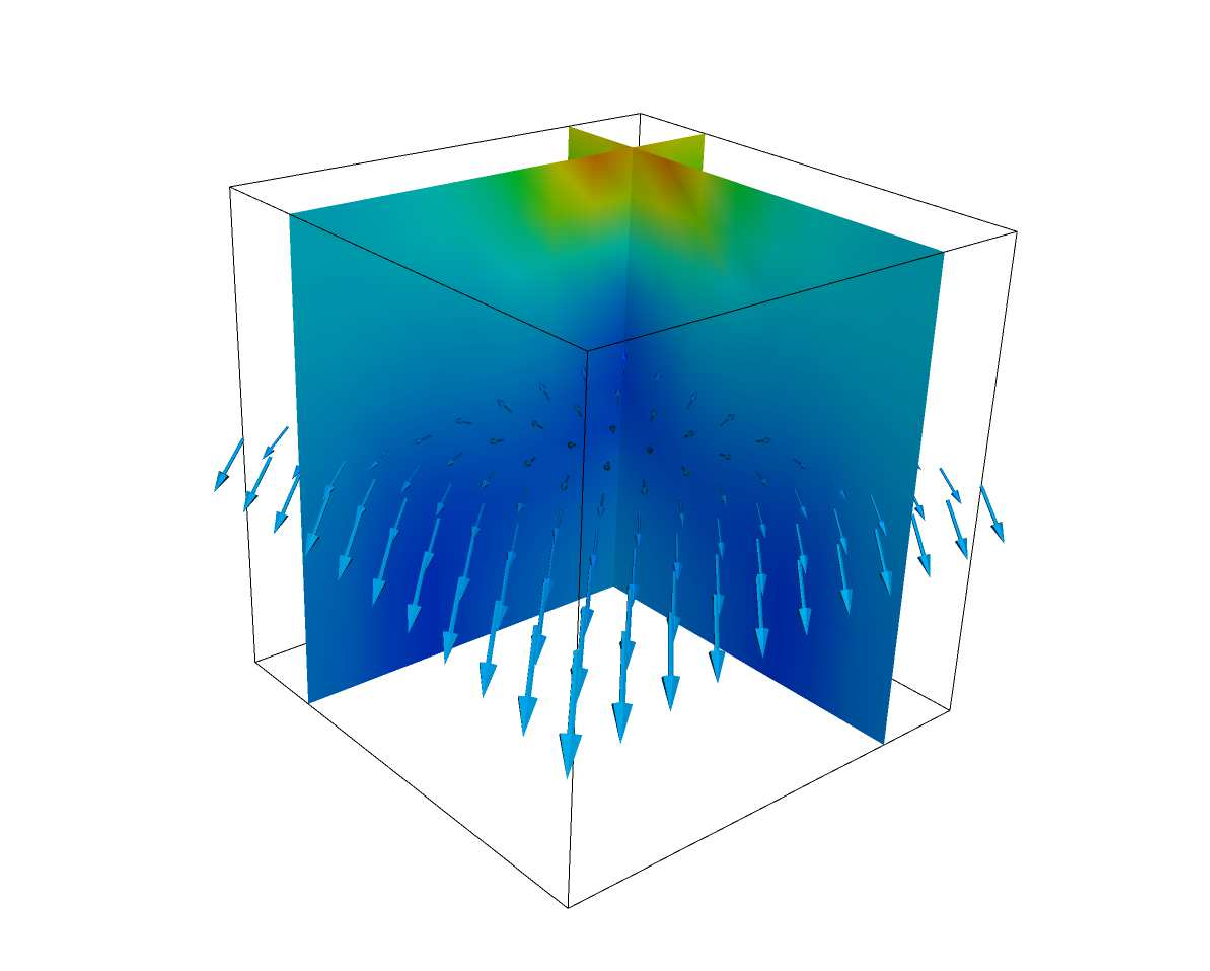
\includegraphics[width=\figwidth]{figures/HeatedBlock}}
\caption{von--Mises Stress and Displacement Vectors.}
\label{HEATEDBLOCK FIG 2}
\end{figure}

Finally the the results can be visualize by calling
\begin{python}
mayavi -d deform.xml -f CellToPointData -m VelocityVector -m SurfaceMap &
\end{python}
Note that the filter \text{CellToPointData} is applied to create smooth representation of the 
von--Mises stress. \fig{HEATEDBLOCK FIG 2} shows the results where the vertical planes showing the 
von--Mises stress and the horizontal plane shows the vector representing displacements.

